\documentclass{article}
\usepackage{graphicx}
\usepackage{amsmath}
\usepackage{polski}
\usepackage[utf8]{inputenc}
\title{UOA ćwiczenie 2}
\author{Denis Firat}
\date{June 2020}

\begin{document}

\maketitle

\section{Cel ćwiczenia}
Celem ćwiczenia jest zapoznanie się z przetwornikiem temperatury TMT 111.

\section{Charakterystyki na podstawie danych pomiarowych}
\subsection{Charakterystyka $I_{wy}=f(temperatury)$}
\begin{figure}[h!]
    \centering
    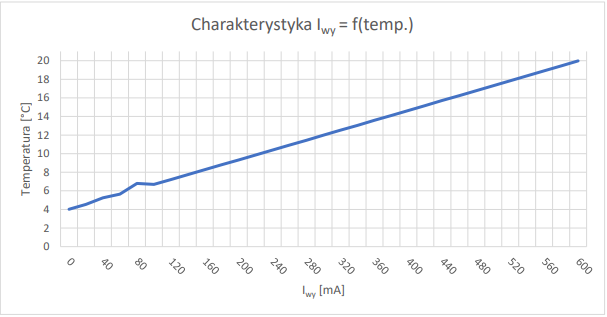
\includegraphics{cw2.png}
    \label{fig:my_label}
\end{figure}\newpage
\subsection{Charakterystyka$I_{wy}=f(R_{obciazenia})$ }
\begin{figure}[h]
    \centering
    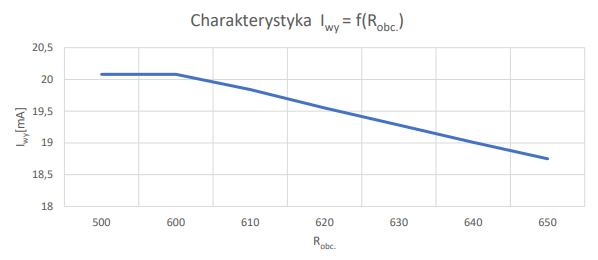
\includegraphics{cw21.png}
    \label{fig:my_label}
\end{figure}



\section{Pytania i odpowiedzi}
\subsection{Sposoby podłączenia czujników do przetworników, wady i zalety}
\begin{figure}[h!]
    \centering
    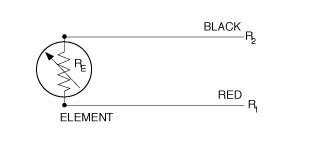
\includegraphics{cw23.jpg}
    \caption{Podłączenie czujnika dwoma przewodami}
    \label{fig:my_label}
\end{figure}
\begin{figure}[h!]
    \centering
    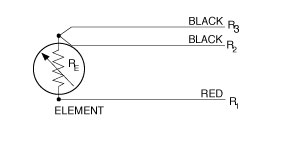
\includegraphics{cw24.jpg}
    \caption{Podłączenie czujnika trzema przewodami}
    \label{fig:my_label}
\end{figure}
\begin{figure}[h!]
    \centering
    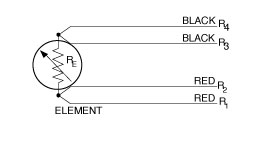
\includegraphics{cw25.jpg}
    \caption{Podłączenie czujnika czterema przewodami}
    \label{fig:my_label}
\end{figure}
Te trzy metody różnią się dokładnością oraz ceną. Jak łatwo się domyśleć im więcej przewodoów użyjemy, tym droższe będzie nasze połączenie.
Zaletą większej ilości przewodów jest dokładność. Podłączenie dwu przewodowe sprawdza się w przypadku krótkich podłączeń(kilka metrów).
Im dłuższy jest przewód tym większe są zakłócenia sygnału mierzonego czujnikiem. Podłączenie trzeciego przewodu kompensuje te zakłócenia i 
zazwyczaj jest to wystarczające. Podłączenie czteroma przewodami zapewnia podwójną kompensację, ale z względu na cene jest rzadko stosowane. 

\subsection{Opisać  jaki to jest przetwornik dwuprzewodowy}
Jest to przetwornik, który połączony jest z czujnikiem z pomocą dwóch przewodów. Jest to najprostszy, a zarazem najgorszy sposób podłączenia.
Przetwornik przetwarza rezystancje czujnika termorezystancyjnego by uzyskać informację o temperaturze otoczenia czujnika. Niestety przewody
posiadają swoją własną rezystancję, która dodatkowo zmienia się wraz z zmianami otoczenia przewodów. Ze względu na szeregową budowę
przetwornika dwuprzewodowego, rezystancje te sumują się. 

\subsection{Wyjaśnić zależność zmiany prądu wyjściowego przetwornika dwuprzewodowego (przy stałym wejściu) , przy zmianie rezystancji obciążenia}
Przetwornik użyty do wykonania pomiarów w tym doświadczeniu nadaje sygnał z zakresu
4…20mA. Wartość natężenia prądu, maleje w sposób liniowy wraz z wzrostem rezystancji obciążenia.

\subsection{Określić maksymalną rezystancję obciążenia  dla klasy dokładności przetwornika  0,1\%}
$$U=R_{obc}\cdot I_{wy}=610\cdot 0,01984=12,1024[V] $$
$$R_{obc.max}=\frac{U}{I_{wy.min}}=\frac{12,1024}{0,004}=3026\pm 3[\Omega]$$
\subsection{Co mierzy ultradźwiękowy przetwornik poziomu}
ultradźwiękowy przetwornik poziomu, mierzy poziom substancji w zbiorniku, najczęściej cieczy,
ale może też mierzyć substancje sypkie. Pomiar dokonywany jest za pomocą ultradźwiękowego czujnika, który
wysyła sygnał w stronę tafli cieczy, a następnie "czeka" na odbity sygnał. Dokonywany jest pomiar
czasu między wysłaniem i odebraniem sygnału. Na podstawie tego czasu i prędkości fali,
obliczana jest odległość między czujnikiem, a poziomem substancji.
\end{document}
